\NativeSlot{41}{86}{%
% p067_s01
\noindent
\ExamTile{.75}{\ExamQuestion{4.}{5}%
剪纸是我国国家级非物质文化遗产，将纸对折后剪出重复的图案是剪纸中最基础的技法。右图是下面（\hspace{1.8em}）项剪出的。\par
}\hfill\ExamTile{.225}{\centering
  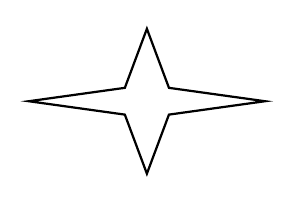
\begin{tikzpicture}[x=1cm,y=1cm,line width=.8bp]
    \draw (-1.5,0)--(-.28,.17)--(0,.92)--(.28,.17)--(1.5,0)--
          (.28,-.17)--(0,-.92)--(-.28,-.17)--cycle;
  \end{tikzpicture}
}\par
\BookFigure{figures/p067_s01-01.tex}
}
\NativeSlot{192}{41}{%
% p067_s02
\ExamQuestion{5.}{5}%
分针从\(6\)走到\(9\)，绕中心点按\mbox{（\hspace{1.8em}）}方向旋转了\mbox{（\hspace{1.8em}）}度。\par
\ExamOptions{A. 顺时针\quad\(30\)}{B. 逆时针\quad\(90\)}{C. 顺时针\quad\(90\)}{D. 逆时针\quad\(30\)}
}
\NativeSlot{263}{131}{%
\ExamGroup{三、画一画。（共68分）}
% p067_s03
% p067_s04
% p067_s05
\ExamQuestion{1.}{5}%
画出下面图形的另一半，使它们成为轴对称图形。（9分）\par
\BookFigure{figures/p067_s03-01.tex}
}
\NativeSlot{451}{65}{%
% p067_s06
% p067_s07
% p067_s08
% p067_s09
\ExamQuestion{2.}{5}%
画出下面图形的对称轴（有几条画几条）。（3分）\par
\smallskip\noindent
\ExamTile{.24}{\BookFigure{figures/p067_s06-01.tex}}\hfill
\ExamTile{.24}{\BookFigure{figures/p067_s07-01.tex}}\hfill
\ExamTile{.24}{\BookFigure{figures/p067_s08-01.tex}}\hfill
\ExamTile{.24}{\BookFigure{figures/p067_s09-01.tex}}\par
}
\NativeSlot{575}{142}{%
% p067_s10
\ExamQuestion{3.}{5}%
按要求画一画。（19分）\par
（1）将下面的图形绕\(O\)点顺时针旋转\(90^\circ\)画出图形，再向右平移\(3\)格画出图形。（6分）\par
\BookFigure{figures/p067_s10-01.tex}
}
